121. \begin{figure}[ht!]
\center{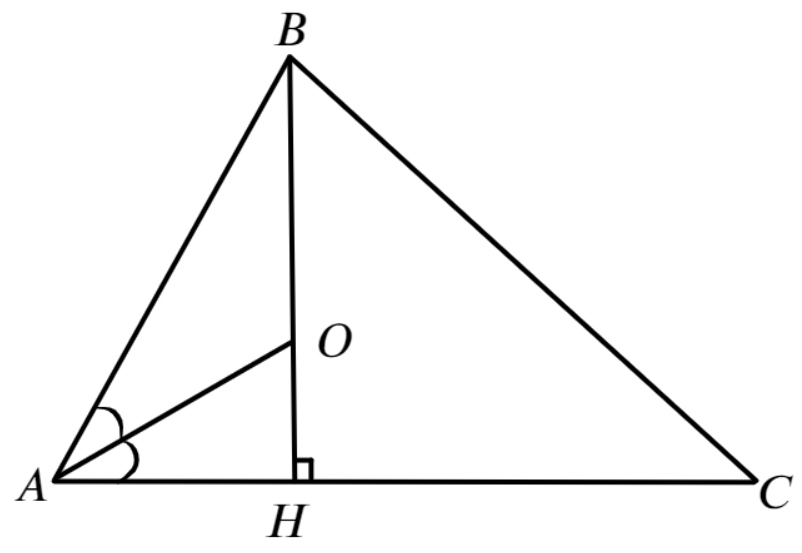
\includegraphics[scale=0.35]{g9-121.png}}
\end{figure}\\
По свойству основания биссектрисы имеем $\cfrac{AB}{AH}=\cfrac{BO}{OH}=\cfrac{5}{4}.$ Тогда $\cos(\angle A)=\cfrac{AH}{AB}=\cfrac{4}{5},\ \sin(\angle A)=\sqrt{1-\cfrac{16}{25}}=\cfrac{3}{5}.$ По теореме синусов для треугольника $ABC$ получим $\cfrac{BC}{\sin(\angle A)}=2R,\ \cfrac{12}{\cfrac{3}{5}}=2R,\ R=10$см.\\
